\section{Introduction}
In this blog post, I will
give a very brief
introduction to Renormalization Group (RG)
theory.

This blog is about quantum computing
and more generally about
quantum information science (QIS).
So why should a person working in QIS
be interested in RG theory?
One reason is that
RG theory describes how
correlation functions
scale, and
correlation functions
are crucial in: (1)the study of quantum entanglement
(2)both classical and quantum Shannon information
theory.

Physicists
like to study how a
theory transforms under a family of operations.
Such families of operations
usually constitute a mathematical group.
The operations might be discrete, as with
PTC (P=parity, T=time reversal, C=charge conjugation)
or continuous (continuous transformations
are a type of generalized rotation). In
the case of the renormalization
group, physicists consider
how a theory transforms under
an operation that ``scales"
 the unit of length.

It's useful (at least to me) to think
of such scaling as a type of
lossy data-compression or
smoothing.
Accordingly,
RG theory can be viewed
as a meta-theory
that describes how theories change under
lossy data-compression. Hence, a
more precise
but less catchy title for this blog post
would have been ``Honey,
I applied lossy data-compression to
 the theory (and the kids)."



\section{Books and other references on RG}
Achtung! There is a huge amount of
literature on RG theory,
and I'm only familiar with
a tiny amount of it,
so don't trust too much my advice
in this section.


My favorite beginner's book on
RG theory is
Ref.\cite{Mc} by McComb.
I like this book a lot,
although I think many aspects of it
could be improved (including
fixing all the typos). This book assumes
very little prior knowledge,
and is very intuitive.

Another book
that I consult occasionally
is Ref.\cite{Go} by Goldenfeld. It's
 a little more advanced
than the book by McComb
and covers some topics not
covered by McComb.

Last but not least,
I recommend Ref.\cite{Sr}
by Srednicki,
an excellent, very comprehensive
 book about
quantum field theory from
a high energy
physics perspective.
This book discusses many topics
besides the RG, but it
includes a nice
explanation of
Feynman diagrams,
renormalization and RG,
all from a high energy
physics point of view.


Taste in physics books is very subjective so
I advise you to inspect the books
I've recommend
and many others besides. Then
form your own opinions.

Besides books, the reference section
at the end of this article also
lists
a few relevant Wikipedia
articles that I found interesting.


\section{RG theory- a big tent}

RG theory is
truly a big tent.
It has been applied in
a wide variety of scientific areas.
Here is a partial list of some of
those areas. Doubtlessly, I've
failed to list
some areas, and new areas
will arise in the future.

\begin{itemize}
\item classical Shannon information theory
\item quantum information science, quantum
Shannon information theory,
study of quantum entanglement.
Density Matrix Renormalization Group (DMRG).
\item
fluid mechanics (turbulence)
\item
chaos and fractal theory
\item
differential equations
\item
statistical mechanics (phase transitions)
\item
probability and statistics
\item
quantum field theory,
both relativistic (used
in high energy physics) and
non-relativistic (used in condensed matter
physics)
\item (as IBM's Watson would say, ???)
computational complexity and algorithms theory,
how the number of
steps in an algorithm depends
on the number of
input bits $n$.
\end{itemize}

\section{What is renormalization?}

The subject of renormalization
methods includes the following topics:
\begin{itemize}
\item regularization:
defining a divergent integral as the
limit of a finite integral.
The parameter than one takes
the limit of is called the
regulator of the integral.
\item renormalization:
a process of possibly
adding a finite number
of new interactions to a field theory
and dividing certain parameters
of the field theory
by normalization constants
so as to make the
field theory finite. These
normalization constants
are parameterized by a
regulator and diverge as
that regulator tends to a
certain value.
\item RG theory: a meta-theory
about how a field theory transforms
under scale transformations.
\item perturbation expansion of a field
theory
\end{itemize}
This article will concentrate
on the topic of RG theory,
but all these topics are closely
related.

Let ``{\bf dofs}" stand for
degrees of freedom.

Note that the word
``scaling" is used in a very
special way
in RG theory.
\emph{Scaling in RG theory =
lossy data-compression
that
reduces the number of dofs of a field theory.}
Some synonyms for ``scaling"
in RG theory:
data-compressing,
screening,
dressing a bare coupling constant,
pruning,
decimating,
averaging,
coarse graining,
smoothing,
forgetting initial conditions,
integrating out ultraviolet dofs,
zooming out,
shrinking. Some antonyms:
zooming in,
magnifying,
expanding,
dilating.

Lossy data-compression
is associated with
 the phenomenon of screening,
whereby a charged particle polarizes
its surrounding medium so that
the charge perceived by
an observer (called
the effective charge)
decreases as
the observer moves
away from the particle.


\section{A whiff of thermodynamics}
RG theory is intimately linked to
thermodynamics,
and thermodynamics is a world in itself.
Here is but a whiff of thermodynamics.
The \textbf{partition function} $Z$ is defined by

\beq
Z = {\rm tr}(e^{-\beta H})
=\sum_j e^{-\beta E_j}
\;,
\eeq
where $H>0$ is the Hamiltonian matrix
of the system, and $\{E_j\}_j$ are the
eigenvalues of $H$.
The \textbf{free energy}
$F$ is defined in terms
of $Z$ by

\beq
-\beta F = \ln Z
\;,
\label{eq-bridge}
\eeq
 where
$\beta = \frac{1}{k_B T}$,
$k_B$ is Boltzmann's constant, and
$T$ is the temperature of the system.
All the thermodynamic observables
can be expressed in terms of
$F$ and it's derivatives with
respect to $\beta$.
McComb calls Eq.(\ref{eq-bridge})
the ``bridge equation",
because it bridges the microscopic physics
with the macroscopic one. Nice name!
One could write volumes about $F$
alone. However, since
this is just a brief article,
let's just point out the interesting fact that
at low temperatures (i.e., high $\beta$),
$F \approx E_1$, where $E_1$ is the
lowest (i.e., ground state)
energy of the system.


\section{An essence of field theory}
In RG theory, one considers
a ``field" (for instance,
a scalar field $\phi(x)\in \RR$
assigned to each point $x\in \RR^d$,
or a spin field $S_i\in\{-1,1\}$
assigned to each point $i$ of a
discrete lattice
embedded in $\RR^d$).


Let $d$ be the number of dimensions of
the space that labels
the field being considered. For
instance, $d=3$
when the field being considered varies over
3 spatial directions but
is stationary (i.e., does not depend on time).
In relativistic quantum field theory,
one is interested in
$d=4$ because a different field
value is attached to each ``event"
(i.e. space-time point).

As is customary in the RG theory literature,
we will use $\epsilon$ to denote

\beq
\epsilon = 4 -d
\;.
\eeq
(Mnemonic: note that the above
equation doesn't change if
you interchange $\epsilon$ and $d$.
The equation $\epsilon = d-4$ (not used here) is
not invariant under the same interchange.)


On a cubic lattice, the separation
in
the $x$ (or $y$ or $z$) direction
between two neighboring lattice points
is called the \textbf{lattice constant}
and will be denoted by $a$.

Field theories are described by
a Hamiltonian. In RG theory, one often
considers the
 Ising Hamiltonian
 and variants thereof.
 The Ising Hamiltonian in $d$ dimensions
 is defined by

\beq
H =
-J\sum_{(i,j)\in\;nn}S_i S_j -
B\sum_{i\in\;lp} S_i
\;,
\eeq
where

\beq
\begin{array}{l}
lp= \mbox{ a set of lattice points
in a hyper-cubic lattice embedded in $\RR^d$},\\
nn=\{(i,j)\in lp: \mbox{$i$
and $j$ are nearest neighbors}\},
\end{array}
\;
\eeq
$S_i\in \{-1,1\}$ for all $i\in lp $.
$S_i$ represents the spin at
lattice point $i$, $J$ is the
spin-spin coupling, and $B$ is
an external magnetic field interacting
with the spins.
One often defines generalized
coupling constants $K_j$ by
$K_1 = \beta J$, $K_2 = \beta B$.

Continuous
instead of discrete field
theories are also frequently
considered in RG theory. For example, the
Hamiltonian for the
$\phi^4$ theory
with mass $m$ and
coupling constant $\lambda$
is given by\footnote{In equation
Eq.(\ref{eq-phi-four}),
$\phi, m, \lambda$ represent
the bare quantities, often
denoted by $\phi_0, m_0, \lambda_0$.}

\beq
H= \int d^dx \left\{\frac{1}{2}
{\sum_{j=1}^d(\partial_j \phi)^2}
+ \frac{1}{2}m^2\phi^2  +
\frac{\lambda}{4!}\phi^4\right\}
\;.
\label{eq-phi-four}
\eeq
One can define generalized
coupling constants here too:
let $K_1 = m^2$ and $K_2 = \lambda$.

A beautiful aspect of
RG theory is that it
applies to any field theory,
be it continuous or discrete,
relativistic (as considered
in high energy physics) or
non-relativistic (as considered
in condensed matter physics).

\section{Naive versus fractal
``scaling" dimensions}



Let the real number $b\geq 1$
denote the {\bf spatial
compression (i.e., spatial scaling) factor}.
Upon compression, the distance $\delta x$
between
any two spatial positions shrinks
to $\delta x'= \frac{\delta x}{b}$.

In
high energy physics, it
is customary to use an
{\bf energy scaling factor}
$b_e = 1/b$. It is
useful to be fluent in both
$b$ and $b_e$ languages.
Since $1\leq b < \infty$,
it follows that
$0<b_e\leq 1$. As
$b$ goes from 1 to $\infty$,
$b_e$ goes from 1 to 0.
$b$ and $b_e$  are both 1 at the same time.
They both start at 1, but one goes up
and the other down.
The point $b=b_e=1$
corresponds to the microscopic,
ultraviolet theory, whereas
the point $b=\infty$, $b_e=0$
corresponds to the macroscopic,
infrared theory.
Note also that
$\ln b_e = -\ln b$
so that as $\ln b$ goes
from 0 to $\infty$,
$\ln b_e$
goes from 0 to $-\infty$.



If one uses Planck units in which
$\hbar = c = 1$, then time and length
have dimensions of $L$,
whereas energy, mass, and momentum
have dimensions of $1/L$. For
a length $x$ and
an energy $E$,
one has

\beq
x' = \frac{x}{b}= b_e x
\;,
\eeq

\beq
E'=\frac{E}{b_e}=bE
\;.
\eeq

A physical quantity $q$
can be assigned both a \textbf{naive dimension} $D_q$
given by dimensional analysis,
and an \textbf{anomalous or fractal dimension}
 $y_q$.
This is expressed with the following notation:

\beq
[q]=L^{D_q}
\;,
\eeq
and\footnote{Our
definition Eq.(\ref{eq-def-fractal})
of fractal dimension $y_q$ is the standard
definition of fractal dimension, namely
log of number of self similar
pieces divided by log of magnification. See
Ref.\cite{wiki-fractal}}

\beq
q'= b^{y_q} q
\;.
\label{eq-def-fractal}
\eeq
For example,
given 3 quantities $q_j$ for $j=1,2,3$, then

\beq
\left[\frac{q_1}{q_2 q_3}\right]=
L^{D_1-D_2-D_3}
\;,
\eeq
and

\beq
\frac{q'_1}{q'_2 q'_3}
= b^{y_1-y_2-y_3}\frac{q_1}{q_2 q_3}
\;.
\eeq

Note that a length $x$ has
$D_x=1$ and $y_x=-1$.
In some cases, it makes sense
to set $y_q=-D_q$ for all quantities $q$.
However, in other
cases, one cannot set $D_q=-y_q$
for all quantities $q$. The cases where one
can (ditto, cannot) set $D_q=-y_q$
for all $q$ are associated with lossless (ditto, lossy)
data-compression. We try to explain
why this is so in Section \ref{sec-corr}.

\section{Real and momentum space RG}
Let $\phi_x\in \RR$
be the value of a field
at position $x\in \RR^d$. For
each $x$, $\phi_x$ is a dof of the
theory. One can also consider
a conjugate dof $\phi_p$
which is the Fourier transform of $\phi_x$.
Only $\phi_p$
for  momenta $p$
in
the ball $\{p: |p|<\Lambda\}$
are allowed.
$\Lambda$,
the maximum momentum magnitude allowed,
 is called the {\bf cutoff
momentum}.


In {\bf real space RG}
applied to a cubic lattice with
lattice constant $a$,
we map
a $d$-dimensional block with sides of length $b a$
into a  block with sides of length $a$.
In so doing, we are
data-compressing the information
assigned to $(b a)^d$ lattice points
into the information assigned to a
single lattice point.
(The information assigned
to a lattice point is the value
of $\phi_x$ or other field
attached to that lattice point.)


In {\bf momentum space RG},
we data-compress by mapping the
information in $\{\phi_p: |p|<\Lambda\}$
into the information in
$\{\phi_p: |p|<\Lambda/b\}$.
This process is often described
by saying that we are
integrating the ultraviolet dofs of the theory.

So what do real and momentum space RG
have in common?
In both real and momentum space RG,
we reduce the number of dofs
 of the theory being considered
from $N_{dofs}$ to $N'_{dofs}$, where

\beq
b = \frac{N_{dofs}}{N'_{dofs}}
\;.
\eeq


\section{Correlations rule the world}
\label{sec-corr}

As before, let
 $\phi_x\in \RR$
be the value of a field
at position $x\in \RR^d$.
 $\phi_x$
is taken to be a random variable.
How the average $\av{\phi_{x_1}\phi_{x_2}}$
decays with distance $r=|x_1-x_2|$
is characterized by a decay length $\xi$
called the \textbf{correlation length}
 of $\phi_x$.



Lossless (ditto, lossy) data-compression
of the theory
is associated with zero (ditto, non-zero)
$\xi$.
The intuition
for this fact is that a field with
$\xi=0$ is composed of
probabilistically independent dofs $\phi_x$,
and therefore pruning those
dofs causes no loss of information.


As mentioned before, in the
case of lossless (ditto, lossy)
data-compression, one can (ditto, cannot)
set the naive and fractal dimensions
 equal (up to a sign) for every
physical quantity (i.e.,
$y_q=-D_q$ for all $q$).

One can prove that there is
a number $d_{uc}$ called
the \textbf{upper critical dimension},
such that $\xi=0$
if $d\geq d_{uc}$.
For instance, for a $\phi^4$
theory, $d_{uc}=4$. For $d\geq d_{uc}$,
one can ``neglect the thermal
fluctuations", set $\xi=0$,
assume lossless data-compression,
and
set $y_q=-D_q$ for all $q$.
The Landau and mean field
models describe this lossless regime.



\section{Renormalization (semi-)group}
Let $b, b_1,b_2,b_3\geq 1$.
If $R_b$ denotes
 data-compression
with compression factor $b$
of a  theory, then clearly

\beq
R_{b_1 b_2} = R_{b_1}R_{b_2}
\;.
\eeq
Note that
$R_1 R_b = R_b$
(identity property),
and  $R_{b_1}(R_{b_2}R_{b_3})=
(R_{b_1}R_{b_2})R_{b_3}$
(associative property).
However, one cannot
set $R_{1/b}R_{b}=R_1$ (inverse property)
because $1/b$ is not greater than 1.
Physically,
the reason RG operations
don't have inverses is
that they represent lossy data-compression,
and therefore are irreversible.
So the set of transformation
$\{R_b: b\geq 1\}$
is not a true mathematical
group. In truth, it only
satisfies the properties of
a weaker algebraic
structure called a semi-group.\footnote{However,
if the theory is scale invariant
as happens when it sits at a critical point,
then
one can consider all $b> 0$,
not just $b\geq 1$,
and the set $\{R_b: b>0\}$
is a true group.}.
Physicists, however, call it a group
anyway.







\section{RG streamlines}
A theory is described by a Hamiltonian
$H$. Each interaction term
in the Hamiltonian is
multiplied
by a different \textbf{generalized c.c. (coupling
constant)} $K_j$
which measures
the strength of that
interaction term. Let
$\vec{K} = (K_1, K_2, \ldots K_{N_{c.c.}})$.
Applying $R_b$ once
gives

\beq
H' = R_b H,\;\; \vec{K}'=R_b\vec{K}
\;.
\eeq
Applying $R_b$ multiple times gives

\beq
H^{(n+1)}= R_b H^{(n)},
\;\;
\vec{K}^{(n+1)}= R_b \vec{K}^{(n)}
\;,
\eeq

\beq
H^{(n)}= R_b^n H^{(0)},
\;\;
\vec{K}^{(n)}= R_b^n \vec{K}^{(0)}
\;,
\eeq
for $n=0,1,2, \ldots$. The
sequence $\vec{K}^{(0)},
\vec{K}^{(1)}, \vec{K}^{(2)}, \ldots$
describes a one-dimensional curve
(a streamline, a flow)
in c.c. space. A different curve
is traced for
each initial condition
$\vec{K}^{(0)}$. The streamlines
flow from $b=1$ to $b=\infty$ (or,
in $b_e$ language,
from $b_e=1$ to $b_e=0$).

\section{Fixed points of the trivial
and critical kind}

If, as $n$ tends to infinity,
\beq
\vec{K}^{(n)}\rightarrow \vec{K}^*
\;,
\eeq
we say $\vec{K}^*$ is a
\textbf{fixed point in the c.c.'s}.
Other functions of $\vec{K}$
like the Hamiltonian $H(\vec{K})$
and the correlation length $\xi(\vec{K})$
also tend to a fixed point

\beq
H(\vec{K}^*)=H^*,
\;\;
\xi(\vec{K}^*)=\xi^*
\;.
\eeq


Note that the correlation length
$\xi$ transforms as

\beq
\xi'=\frac{\xi}{b}
\;,\;\;
\xi^{(n)} = \frac{\xi^{(0)}}{b^n}
\;.
\label{eq-xi-zero-to-n}
\eeq
Therefore, for large $n$,
\beq
\xi^* = \frac{\xi^*}{b^n}
\;.
\label{eq-xi-lim}
\eeq
Eq.(\ref{eq-xi-lim}) has two possible solutions.
Either $\xi^* = 0$, in which case
we say the fixed point $\vec{K}^*$
is trivial, or $\xi^* = \infty$,
in which case we say the fixed point
is critical.


\textbf{Trivial fixed points} are not
very interesting. Since they
have $\xi^*=0$, they can be understood
in terms of
lossless data-compression and
naive dimensions for the c.c.'s.

\textbf{Critical points}
are much more interesting.
Since they
have $\xi^*=\infty$, they can be understood
in terms of
lossy data-compression
and fractal dimensions for the c.c.'s.

Two examples of critical points that
occur in nature are the Curie temperature of
an Ising system (the temperature
at which the magnetization of the
system goes from
zero to growing, spontaneously, at zero
externally applied magnetic field).
Another showcase critical point is
the critical point of water (a
unique point in the PVT phase diagram
of water, a point at which gaseous and liquid
water coexist). The temperature at which
a critical point occurs
is called its {\bf critical temperature}
and is
denoted by $T_c$.
Critical points are also sometimes
called second
order phase transitions.


\section{Critical exponents and universality classes}
How various thermodynamic
quantities behave near and precisely
at a critical point is described
by a slew of
{\bf critical exponents}.
It is common to define
6 critical exponents $\alpha, \beta,
\gamma, \delta,\nu ,\eta$ (all defined
so as to be non-negative)
defined on page 150 of McComb.
One
can use very general
thermodynamic arguments to prove
that these 6 exponents must satisfy
4 simple relationships
between them. Thus,
one need only calculate 2 of
6. The 2 that are usually calculated
are
$\nu$ and $\eta$.

$\nu$ and $\eta$
can both be inferred
from the behavior of Greens's functions.
Let $\phi_x$ be the value of
a field at point $x$. Let
$\av{Q}$
denote the average of a
quantity $Q$. We will use the
following shorthand notations

\beq
r= |x_1-x_2|,\;\;
\Delta\phi_x = \phi_x - \av{\phi_x},\;\;
\theta_c = \frac{\Delta T}{T_c}=
\frac{T-T_c}{T_c}
\;.
\eeq
We define the {\bf Greens's function} $G(r)$
by

\beq
G(r) = \av{\phi_{x_1}\phi_{x_2}}
\;,
\eeq
and the \textbf{connected Greens's function}
 $G_c(r)$ by

\beq
G_c(r)=
\av{\Delta\phi_{x_1}\;\;\Delta\phi_{x_2}}
=
\av{\phi_{x_1}\phi_{x_2}}
-\av{\phi_{x_1}}\av{\phi_{x_2}}=
 \av{\phi_{x_1},\phi_{x_2}}
\\
\;.
\eeq
The behavior of $G_c(r)$ near but not precisely
at a critical point is of an
exponential form, with decay
constant give by the correlation length $\xi$.
The dependance of $\xi$ on temperature
determines the critical exponent $\nu$:

\beq
G_c(r)\sim \exp(-r/\xi),
\;\;
\xi = |\theta_c|^{-\nu}
\;.
\eeq
(Note that for $\nu>0$,
$\xi\rarrow \infty$ as $T\rarrow T_c$.)
The behavior of $G_c(r)$ precisely at
a critical point is an inverse power
law, and the power of the law
determines the critical exponent $\eta$:


\beq
G_c(r)\sim 1/r^{pow},\;\;pow = d-2+\eta
\;.
\eeq
(Let $d=4$. If $\eta=0$, this gives
an inverse square law. If $\eta>0$,
$G_c(r)$ decays faster than
when $\eta=0$,
as one expects if there is screening.)

For all
field theories, all critical points
with the same critical exponents
 are
said to be in the same
\textbf{universality class}.
For example, the $\phi^4$ theory
has a single trivial fixed point for $d\geq 4$,
but for $d\leq 4$,
it has a single critical fixed
point, called the Wilson-Fisher point,
which has the same critical exponents
as the critical point
of the Ising model in $d$ dimensions.

Universality classes are few and far between
because theories are scale invariant
at a critical point,
and scale invariant theories are
few and far between.



\section{Relevant, marginal and irrelevant operators}

It is interesting
to analyze the behavior
of a field theory in the vicinity
of a critical point.
To do this, it
is convenient to replace
the
generalized c.c.'s
$\vec{K}=(K_1, K_2,\ldots, K_{N_{c.c.}})$
by \textbf{natural c.c.'s}
$\vec{g}=(g_1, g_2,\ldots, g_{N_{c.c.}})$.
The natural c.c.'s are natural
coordinates for describing
the particular
critical point
being considered. They
have the critical point as their origin
(i.e., $\vec{g^*}=0$).

The set of all points that flow into
 the critical point (i.e., the ``basin
of attraction" of the critical point)
is called the \textbf{critical surface}.
As a consequence
of Eq.(\ref{eq-xi-zero-to-n}),
all points in the critical surface
have infinite correlation length $\xi$,
just like the critical point
itself (in
a manner of speaking, they get
infected by the critical point).


Note that
\beq
g_j' = b^{y_j} g_j,
\;\;
g_j^{(n+1)} = b^{ny_j} g_j^{(0)}
\;
\eeq
for all $j$. Since $b\geq 1$, there
are three possible scenarios for each
$g_j$:
\begin{itemize}
\item $y_j>1$:
In this case
$g_j^{(n)}\rarrow \infty$
as $n\rarrow \infty$. We say
$g_j$ is a relevant c.c..

\item $y_j<1$:
In this case $g_j^{(n)}\rarrow 0$
as $n\rarrow \infty$. We say
$g_j$ is an irrelevant c.c..
\item $y_j=1$:
In this case $g_j^{(n)}$ tends to a constant
as $n\rarrow \infty$. We say
$g_j$ is a marginal c.c..
\end{itemize}
If an  interaction term in the
Hamiltonian is multiplied by a relevant c.c.,
we call that interaction term a relevant
operator, and likewise for irrelevant and marginal.

\begin{figure}[h!]
\centering
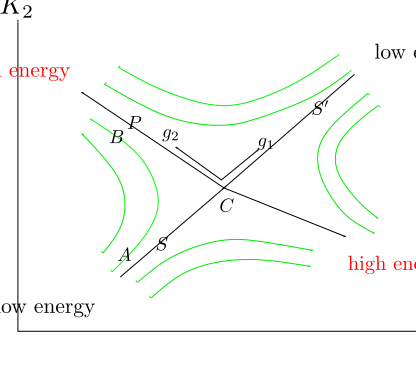
\includegraphics[height=2.7in]
{renorm-group/renorm-group-critical-point.png}
\caption{RG streamlines in
    the vicinity of a critical point
    for a theory with 2 coupling constants.}
\label{fig-rg-critical-point}
\end{figure}



Fig.\ref{fig-rg-critical-point} shows the typical behavior
of the RG streamlines in the vicinity
of a critical point, assuming $N_{c.c.}=2$.
In Fig.\ref{fig-rg-critical-point}, point $C$
is the critical point.
The $K_1,K_2$ axes are for the generalized
c.c.'s and the $g_1, g_2$
axes are for the natural c.c.'s.
The arrows on the streamlines point
in the direction of
increasing $b$ (i.e., decreasing $b_e$).
In the case of Fig.\ref{fig-rg-critical-point},
the critical surface
is a
one dimensional curve, the one that contains
points
$S$, $C$ and $S'$.
No streamlines ever cross the
critical surface. They stay for all $b$
either above or below the critical surface.

If the initial conditions
are such that the theory starts
somewhere on the critical surface,
then for $b$ large enough,
the theory ends at point $C$ where
$g_1=g_2=0$. On the
other hand, if the theory
starts at a point such as $A$
which is close
to the critical surface but not on it,
then the irrelevant c.c. $g_1$ (ditto,
relevant c.c. $g_2$)
shrinks (ditto, grows)
monotonically
as $b$ grows.
By the time the theory reaches, say,
point $B$,
$g_1$ is negligible,
and
$g_2$ is starting to become uncomfortably
large for expanding in powers of it.
A good place to do
 perturbation
theory
is in the vicinity of point $P$,
where the irrelevant c.c. $g_1$
is negligible, and the relevant c.c $g_2$
is much smaller than 1, but still non-zero.


\section{Self-similar coupling constants and beta functions}

Consider
a critical point
with natural c.c.'s
$\vec{g} =(g_1, g_2, \ldots,
g_{N_{c.c.}})$.
Define the fractal
dimension $y_j$ of the c.c. $g_j$ by

\beq
\frac{d\ln g_j}{d\ln b}=
y_j
\;.
\label{eq-dif-yj}
\eeq
In high energy physics, it
is common to
use, instead of $y_j$, a so called
\textbf{beta function} $\beta_j$
defined by

\beq
\frac{dg_j}{d\ln b_e}=
\beta_j
\;.
\label{eq-dif-betaj}
\eeq
Comparing of Eqs.(\ref{eq-dif-yj})
and (\ref{eq-dif-betaj})
and using $\ln b = -\ln b_e$,
one finds

\beq
\beta_j = -g_j\;y_j
\;.
\eeq

Precisely at the critical point
(i.e., at $\vec{g}=0$),
one must have
$\beta_j=0$.
Amazingly, in the vicinity of
the critical point, the
beta function
$\beta_j$ must be of the
form\footnote{When $\epsilon=0$,
the expansion
of  the beta function
in powers of $g_j$
usually starts
at order($g_j^2$).
This is why. The value of $a_{j1}$ (i.e., the order($g_j^1$)
coefficient in the expansion
of the beta function
in powers of $g_j$)
must equal the naive dimension of
$g_j$. As explained in Section
\ref{sec-regulator}, one usually introduces
a renormalization-point mass
 $\mu$ to make $[g_j]=L^0$.
If this is done, $a_{j1}$
becomes proportional to $\epsilon$,
and vanishes when $\epsilon=0$.
}

\beq
\beta_j = \beta_j(g_j, \epsilon)=
a_{j1}(\epsilon) g_j
+ a_{j2}(\epsilon) g_j^2
+ a_{j3}(\epsilon) g_j^3
+\cdots
\;,
\label{eq-beta-g-exp}
\eeq
where the
coefficients $a_{jk}$
are functions only of $\epsilon$,
not of $b_e$. Furthermore, one
must have

\beq
\lim_{\epsilon\rarrow 0}\beta_j= \mbox{ finite number}
\;.
\eeq


Eqs.(\ref{eq-dif-betaj})
and (\ref{eq-beta-g-exp}) yield
an easy to
solve, separable differential equation. Hence,
given $g_j$ and
$\ln (b_e'/b_e)$, one can find the value of
$g'_j$.
One describes this felicitous property
by saying that the c.c. $g_j$ is self-similar
or by saying the humorous
statement that $g_j$
is a ``running c.c.".


More generally, if the
theory has a set of
generalized c.c.'s
$\vec{K} =(K_1, K_2, \ldots,
K_{N_{c.c.}})$
that are not associated with
a particular critical point,
one can still define beta
functions $\beta_j(b_e)$
by

\beq
\frac{dK_j}{d\ln b_e} = \beta_j(b_e)
\;.
\label{eq-dif-kj}
\eeq
Then a fixed point
in the c.c.'s is defined as
any point $\vec{K}^*$
at which $\beta_j=0$
for all $j$.
If $\vec{K}^*$ occurs
when $b_e=0$ (ditto, $b_e=1$),
we call it an infrared (ditto, ultraviolet)
fixed point.\footnote{Some
might be puzzled
by the fact that
we speak of $b_e$
as if it were an energy,
although, in reality, it is
a {\it ratio} of energies.
If the theory has a lattice
constant $a$, define $x_{min} =a$
and $E_{max} = 1/a$. Recall
that $b_e= E/E'$. If we
keep $E'$ fixed at $E'=E_{max}$,
then $b_e$
and $E$ are proportional to each
other.}
For instance, QED (Quantum Electrodynamics)
has $\beta>0$ which gives it
an infrared fixed point,
whereas QCD (Quantum Chromodynamics)
has $\beta<0$ which gives it an ultraviolet
fixed point.

\section{The regulator and the fiducial
mass scale}
\label{sec-regulator}

A continuous
quantum field
theory has
infinite
terms in its perturbation
expansion. That's
not surprising because
such a theory
describes infinitely many
harmonic
oscillators, and each of
those harmonic oscillators  has a
finite zero-point energy of $\hbar\omega/2$.
One regulates the infinities
of a quantum field theory
by introducing a \textbf{regulator}
parameter with a ``catastrophic" value.
The
infinities go away if
the regulator is slightly
off from its catastrophic
value, and they come back as
 the regulator
tends to its catastrophic
value.  All
observable
quantities must
be independent of the regulator.
The two most popular
regulators in the high
energy physics literature
are
\begin{enumerate}
\item
a momentum cutoff $\Lambda$. This
is called Pauli-Villars regularization.
\item
$\epsilon = 4 -d$. This is called
dimensional regularization.
\end{enumerate}

In case (1), the space-time
dimension $d$ is kept
fixed at an integer value, whereas
in (2), $d$ varies
over a continuum of real
numbers.

In case (2), in order to make
the c.c.'s dimensionless,
one needs to introduce a
\textbf{fiducial mass scale}.\footnote{
That's my own name for it, invented
after reading a credit card contract.}
This fiducial mass scale,
called
the \textbf{renormalization-point},
is usually denoted by $\mu$.\footnote{
For those who have studied quantum
field theory previously, let me remind
you of how the
renormalization-point $\mu$ arises.
The c.c. $g$
is replaced by $\mu^p g$
where the power $p$
is chosen so as to make $g$
dimensionless.
$[(d^dx) (\partial \phi)^2]=L^0$
implies $[\phi]= L^{1-\frac{d}{2}}$. Then
$[(d^dx)  \mu^p (g\phi^n)] = L^0$ with
$[g]=L^0$ and $[\mu]=L^{-1}$
implies $d -p +n(1-\frac{d}{2})=0$.
Hence, $p=d(1-\frac{n}{2}) + n$.
For example, in the $\phi^3$
theory in 6 dimensions considered
in Srednicki's book Ref.\cite{Sr},
one gets, using $d = 6-\epsilon$, that
$p= -(6-\epsilon)\frac{1}{2} + 3
= \frac{\epsilon}{2}$.}
In both cases (1) and (2), we need to
introduce a fiducial mass scale,
$\Lambda$ in case (1) and $\mu$ in case (2).
Roughly speaking,
the fiducial mass scale
parameterizes
how we
subtract the infinite
part of the answer.
In case (1),
$\Lambda$ acts both as
the regulator parameter and
the fiducial mass scale.
In case (2), these
two roles are assigned to
separate parameters, $\epsilon$
becomes the regulator and
$\mu$ the fiducial mass scale.

High energy physicists
usually do not use a scaling factor
like $b_e$ or $b$. Instead, they
use $\ln \mu$ (or $\ln \Lambda$)
en lieu of $\ln b_e$
in Eq.(\ref{eq-dif-kj}).
That's no problem. Just replace
$\mu$ by $b_e \mu$ (or
$\Lambda$ by $b_e \Lambda$).
If you keep $\mu$
(or $\Lambda$) fixed and
allow $b_e$ to vary, then
$d\ln(b_e\mu)$ (or $d\ln(b_e\Lambda)$ )
can be replaced by $d\ln b_e$.

\section{RG theory has its pi-groups too!
Callan-Symanzik Type Equations}

In doing dimensional
analysis (Ref.\cite{wiki-da})
for a given problem, one
usually begins by finding the
 pi-groups relevant to the
problem. A pi-group (so called
because the symbols $\pi_1, \pi_2, \ldots$
are used to represent them)
is a product
of quantities that is dimensionless:
\beq
[\mbox{dim-analysis pi-group}]=L^0
\;.
\eeq
Analogously, in RG theory, one
can often identify certain compound
quantities which must be scale
invariant (i.e., independent
of $b_e$).
I like to call such
quantities RG pi-groups.

\beq
\frac{d}{d\ln b_e}
\{\mbox{\rm RG pi-group}\}=0
\;.
\label{eq-callan}
\eeq
The Callan-Symanzik equation
used in high energy physics is
just a special case of Eq.(\ref{eq-callan}).



\section{Forgetting initial conditions.
Are we cheating with infinities?
Where did the infinities go?}

Sometimes it is useful
to have infinities in the
initial conditions of a problem.
For example, it's
useful to use a Dirac delta function
as initial conditions
for a diffusion equation
(or for the differential
equation obeyed by a Greens's function).
The infinities in the initial
conditions are `` forgotten"
 at later times,
as the solution spreads.

A similar situation occurs with
quantum field theories. One starts
with bare c.c.'s like $\phi_0, m_0, \lambda_0$
and these evolve to dressed c.c.'s
like $\phi, m, \lambda$.
The bare
c.c.'s correspond to $\vec{K}^{(0)}$
at ultra-high energy scales $b_e= b=1$.
The dressed c.c.'s
 correspond to $\vec{K}^{(n)}$
for a large $n$
and not-so-ultra-high energy scales,
$b_e\in (0,1)$ but $b_e<<1$.
The bare c.c.'s are
infinite, but never mind, they are
quickly forgotten.
They are forgotten
because the c.c.'s are self-similar,
so we can find $g'$ given
$g$ and $\ln(b'_e/b_e)$.
If $g$ is set
to its bare value $g=g_0$,
then $g$ and therefore $g'$
will be infinite, but
we never set $g=g_0$.

Note that by the same
token, any theory which
has infinite initial conditions
which are forgotten,
can be regulated with a regulator,
and a fiducial mass scale, call it $\mu$. Then
$\mu$ can be replaced
by $b_e\mu$ with $b_e\in(0,1)$,
and RG theory can be used.
The upshot is that any
theory with infinite initial
conditions which are forgotten
is amenable to analysis
via RG theory.




\section{The many faces of a renormalizable theory}

When high energy physicists
talk about a \textbf{renormalizable theory},
their definition
of what that means keeps changing.
Several popular definitions are
\begin{enumerate}
\item
A theory that yields finite
predictions for the observables
when those observables are expressed
as perturbation
expansions in powers of the c.c.'s.
\item
A theory for which only
a finite number of c.c.'s are needed
in order to achieve finite predictions
for the observables.
\item
A theory for which the c.c.'s are self-similar.
\item
A theory for which the
c.c.'s are dimensionless
when $\epsilon=4-d=0$. (Otherwise,
cross-sections blow up at high energies).
\end{enumerate}
So which one is it?
One great insight of RG theory is
that all these definitions are
roughly equivalent. These
properties
are all symptoms of
a field theory that is in the
vicinity of a critical point.
